\subsection{Pile-Up}
\label{subsection: charged particle event multiplicity, pile-up}

The pile-up contribution to the charged particle event multiplicity is approximated as consisting of the distribution from events with a single proton-proton collision and the convolution of two single proton-proton collisions. The average number of proton-proton interactions is given by equation \ref{equation: mu approximation} for small $\mu$ shown in section \ref{subsection: charged particle density, pile-up}. This means the data is dominated by single proton-proton interactions and may be approximated by,

\begin{equation}
	N_\mathrm{observed}(n) \approx \frac{N_\mathrm{single}(n) + \frac{\mu}{2} N_\mathrm{single}(n) \ast N_\mathrm{single}(n)}{A}
	\label{equation: pile-up multiplicity composition}
\end{equation}

with,

\begin{equation}
	N_\mathrm{single}(n) \ast N_\mathrm{single}(n) = \sum_{k=0}^{n} N_\mathrm{single}(k) \cdot N_\mathrm{single} (n - k)
\end{equation}

$A$ is a normalisation constant given by,

\begin{equation}
	A = \sum_{n=0}^{n_\mathrm{max}} N_\mathrm{single}(n) + \frac{\mu}{2} N_\mathrm{single}(n) \ast N_\mathrm{single}(n)
\end{equation}

 $N_\mathrm{observed}(k)$ is the number of events with $n$ charged particles consisting of contributions of events with one or two proton-proton interactions; $N_\mathrm{single}(k)$ is the number of events with $n$ charged particles from single proton-proton interactions, $k$ is the number of charged particles from a secondary proton-proton interaction in an event with $n$ charged particles and $N_\mathrm{single}(k) \ast N_\mathrm{single} (n - k)$ is the convolution of two single proton-proton interactions producing $n$ charged particles. The normalisation constant $A$ may also be expressed as,

\begin{equation}
	A = 1 + \frac{\mu}{2}
\end{equation}

since $N_\mathrm{single}(n)$ and $N_\mathrm{single}(n) \ast N_\mathrm{single}(n)$ are normalised functions of $n$. Solving equation \ref{equation: pile-up multiplicity composition} for $N_\mathrm{single}$ gives,

\begin{equation}
	N_\mathrm{single}(n) = (1 + \frac{\mu}{2}) N_\mathrm{observed}(n) - \frac{\mu}{2} N_\mathrm{single}(n) \ast N_\mathrm{single}(n)
\end{equation}

The form of this equation suggests an iterative procedure may be used in order to approximate $N_\mathrm{single}$, using this approach gives,

\begin{equation}
	N_\mathrm{single}''(n) = (1 + \frac{\mu}{2})N_\mathrm{observed}(n) - \frac{\mu}{2} N_\mathrm{single}(n)' \ast N_\mathrm{single}(n)'
\end{equation}

where $N_\mathrm{single}'(n)$ is an approximation of $N_\mathrm{single}(n)$ and $N_\mathrm{single}''(n)$ is the next iteration of the approximation of $N_\mathrm{single}(n)$. Starting with $N_\mathrm{observed}(n)$ as the initial seed for the process gives the results shown in figure \ref{fig: n single approximation}. The pile-up correction for high multiplicities are not included due to the poor statistical significance at high multiplicities.

\begin{figure}
	\centering
	\begin{subfigure}{0.49\textwidth}
		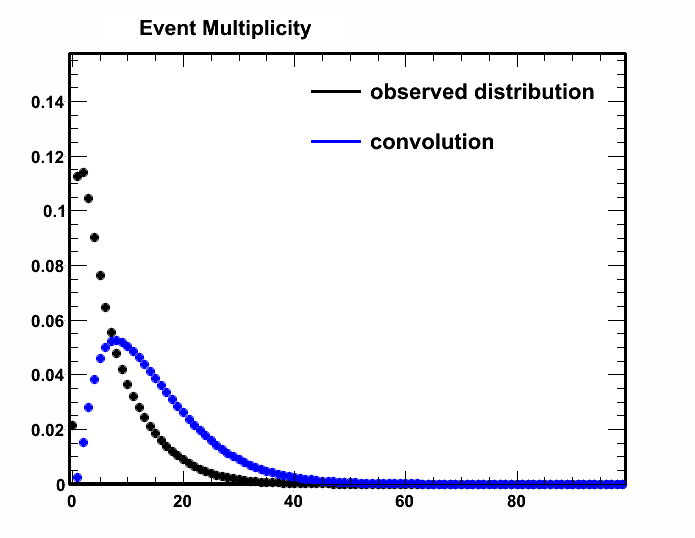
\includegraphics[width=\textwidth]{Chapters/multiplicity/charged_particle_event_multiplicity/images/comparison.png}
		\caption{A comparison of the observed event multiplicity to the convolution of the observed event multiplicity}
		\label{fig: convolution}
	\end{subfigure}
	\begin{subfigure}{0.49\textwidth}
		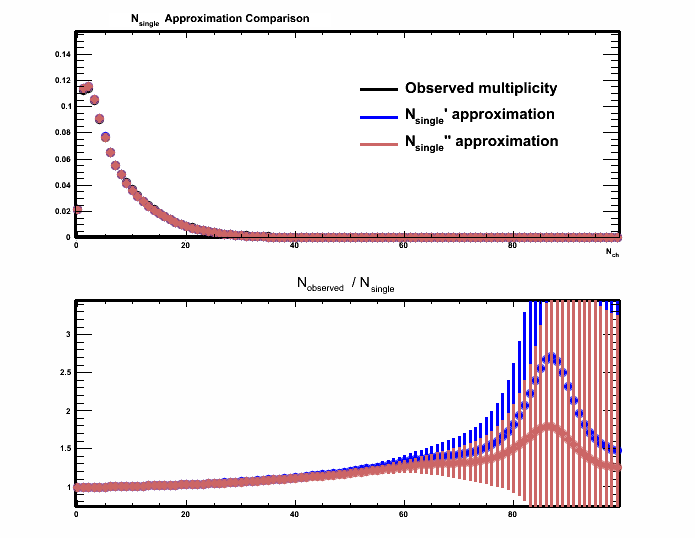
\includegraphics[width=\textwidth]{Chapters/multiplicity/charged_particle_event_multiplicity/images/n_single_approximation_comparison.png}
		\caption{$N_\mathrm{single}$ approximation. The observed distribution is shown in black, the first and second iterations are shown in blue and red respectively.}
		\label{fig: n single approximation}
	\end{subfigure}
	\caption{Pile-up contributions to the charged particle event multiplicity for $2.0 \le \eta \le 4.5$.}
\end{figure}

%Introducing a trigger condition which accepts only events with visible interactions gives the average number of interactions in triggered events i.e. the pile-up ($\mu_1$) as,
%
%\begin{equation}
%	\mu_1 = \frac{\sum^{\infty}_{k=1}{k\cdotp_k}}{\sum^{\infty}_{k=1}{p_k}} = \frac{\sum^{\infty}_{k=0}{k\cdotp_k}}{\sum^{\infty}_{k=1}{p_k}} = \frac{\mu}{1-p_0} = \frac{\mu}{1 - e^{-\mu}}
%\end{equation}
%
%
%
%\begin{equation}
%	\mu_1 \approx \frac{\mu}{1 - (1 - \mu + \mu^2/2)} \approx 1 + \frac{\mu}{2}
%\end{equation}

%At the LHCb detector pile-up is defined as the average number of proton-proton interactions ($n$) in visible events. 

%The number of visible proton-proton interactions ($n$) per bunch crossing follows a Poisson distribution,
%
%\begin{equation}
%	P(n; \mu) = \frac{\mu^n e^{-\mu}}{n!}
%\end{equation}
%
%where $\mu$ is the expected number of visible proton-proton interactions per punch crossing. The pile-up ($\mu_1$) is defined as the 0 suppressed expectation value, for $n \ge 1$, given by (see appendix \ref{AppendixA}),
%
%\begin{equation}
%	\mu_1 = \frac{\mu}{1-e^{-\mu}}
%\end{equation}
%
%$\mu$ is calculated as 0.002 for magnet down data in 2010, see section \ref{subsection: estimation of mu}.
%
%To calculate the multiplicity distribution for events with single proton-proton interactions it is required to correct for effects due to the pile-up. The observed multiplicity distribution ($\theta$) is postulated to be a convolution of single proton-proton interaction distributions ($\phi$), given by,
%
%\begin{equation}
%	\theta(n) = \frac{1}{\sum_{k=1}^{\infty} P(k)} \sum_{k=1}^{\infty}P(k)\phi_k(n)
%\end{equation}
%
%with,
%\begin{equation*}
%	\phi_k = \phi \ast \phi ... \ast \phi \mathrm{\,\,\,\,\,} k \mathrm{\,times}
%\end{equation*}
%
%For small values of $\mu$ it is sufficient to consider only the first two terms. The expression for the pile-up ($\mu_1$) in this regime can be expanded as,
%\begin{equation}
%	\mu_1 \approx \frac{\mu}{1 - (1 - \mu + \mu^2/2)}
%\end{equation}
%or,
%\begin{equation}
%	\mu_1 \approx 1 + \frac{\mu}{2}
%\end{equation}
%
%The expression for the observed distribution in terms of convolutions of single proton-proton interaction distributions approximates to,
%
%\begin{equation}
%	\theta(n) \approx \frac{P(1)\phi(n) + P(2)\phi_2(n)}{P(1) + P(2)} = \frac{\phi(n) + (\mu/2)\phi_2(n)}{1 + \mu/2}
%\end{equation}
%
%In terms of the single proton-proton interaction distribution $\phi$ this is,
%
%\begin{equation}
%	\phi(n) = (1 + \frac{\mu}{2})\theta(n) - \frac{\mu}{2}\phi_2(n)
%\end{equation}
%
%The form of this equation suggests an iterative approach to calculating the solution with,
%
%\begin{equation}
%	\phi^{i+1}(n) = (1 + \frac{\mu}{2})\theta(n) - \frac{\mu}{2}\phi_2^{i}(n) \mathrm{\,\,\,\,\,\,\,\,for\,\,the\,\,} i^{th} \mathrm{\,\,iteration}
%\end{equation}
%
%Since $\mu$ is small a suitable choice at the initial seed for $\phi^0$ is the observed multiplicity $\theta$, this gives the first iteration of $\phi$ as,
%
%\begin{equation}
%	\phi' = (1 + \frac{\mu}{2})\theta - \frac{\mu}{2}\theta_2 = \theta + \frac{\mu}{2}(\theta - \theta_2)
%\end{equation}
%with,
%\begin{equation*}
%	 \theta_k = \theta \ast \theta ... \ast \theta \mathrm{\,\,\,\,\,\,\,\,} k \mathrm{\,\,times}
%\end{equation*}
%
%and for the second iteration,
%
%\begin{equation}
%	\phi'' = \phi' - \frac{\mu^2}{2}(\theta_2 - \theta_3) + \frac{\mu^3}{8}(\theta_2 - 2\theta_3 + \theta_4)
%\end{equation}
%
%The pile-up correction applies only two iteration, the next iteration affects only the $\mu^3$ term which has a small effect on the overall correction due to the smallness of $\mu$.